\documentclass[10pt,letterpaper]{article}
\usepackage{geometry}
\geometry{margin=1in}
\usepackage{graphicx}
\usepackage{tabularx}
\usepackage{booktabs}
\usepackage{enumitem}
\usepackage[table]{xcolor}
\usepackage{multirow}
\usepackage{tikz}
\usepackage{longtable}
\usepackage{array}

\setlength{\parindent}{0pt}
\setlength{\parskip}{0.5em}

%make lists tighter
\usepackage{enumitem}
\setlist{nolistsep}

%reduce spacing before and after section
\usepackage{titlesec}
\titlespacing\section{0pt}{6pt}{0pt}

\title{Lab 1 - PECARN TBI Data, STAT 215A, Fall 2026}

% submission must not contain your name
% but feel free to make a version for yourself with your name on it
\author{}

\begin{document}
\maketitle

\section{Introduction}\label{introduction}

As pointed out in Kuppermann et al. [1], traumatic brain injury (TBI) is a leading cause of death and disability in children. In order to identify TBI, a non-contrast head computed topography (CT) scan is the gold standard diagnostic tool, but it is not without risks. CT scans expose patients to ionizing radiation, which can increase the risk of developing cancer, especially in children under the age of two. CT scans are also expensive and difficult to access in some areas, i.e., rural areas. As of 2006 (the concluding time of the original data collection), there were no widely accepted clinical guidelines for determining which children presenting to the emergenct department with head trauma should receive a CT scan. This work aims to conduct a similar analysis to Kuppermann et al. [1] in order to identify children at very low risk of clinically important traumatic brain injury so that unnecessary CT scans can be avoided. From data cleaning to modeling, this report hopes to provide a comprehensive exploratory data anlysis, cleaning procedure, and decision-modeling to compare with the now established Clinical Decision Rules (CDR) for pediatric head trauma.

\section{Data}\label{data}

This data set is from the Pediatric Emergency Care Applied Research Network (PECARN) and contains information on children ($<18$ years old) who presented to the emergency department with head trauma. The data set includes demographic information (including age, sex, and race), clinical features (including GCS scores, altered mental status (\texttt{AMS}), and loss of consciousness (\texttt{LOC})), and outcomes related to traumatic brain injury (TBI). The outcome variable of interest is \texttt{ciTBI}, which indicates whether the child had a clinically important traumatic brain injury for the purposes of determining the need for CT scans, balancing the risks and benefits of imaging. The data was collected from 25 pediatric emergency departments across the United States between 2004 and 2006 and contains a total of $42,412$ children, with $376$ cases of ciTBI. 

\subsection{Data Collection}\label{data-collection}

The data was collected by multiple different trained site investigators and physicians from 25 different pediatric emergency departments. There were pre-established inclusion and exclusion criteria for the data set (e.g., exclude those who had a GCS score less than 14, those who had trivial injury mechanisms with no signs or symptoms of head trauma, those who had pentrating trauma, those with known brain tumors, those with outside neuroimaging, and those who had pre-existing neurological disorders). Everyone eligible to enroll in this study did not register.

Several variables (e.g., amnesia, heachache, and dizziness) were not collected for children under 2 years old, as these children are unable to communicate such symptoms. Most variables were collected as \texttt{Yes} or \texttt{No} for presenting a certain symptom during their assessment. Some variables were ordinal in nature, representing different levels of that particular variable. All data was recorded on a standardized form for consistency (see Table 1). To test inter-rater reliability, 4\% of patients at each hospital had multiple independent assessments done within 60 minutes of one another.

\begin{table}[htbp]
\footnotesize
\centering
\caption{Case report form adapated from Kuppermann et al. [1].}
\label{tab:form}
\begin{tabularx}{\textwidth}{>{\bfseries\hsize=0.3\hsize}X X}
\toprule
Category & Variables and Items \\
\midrule
Mechanism of injury & 
\begin{itemize}[leftmargin=*, nosep]
    \item Occupant in motor vehicle crash (with documentation of ejection, rollover, death of other passenger, speed, restraint use)
    \item Pedestrian struck by vehicle
    \item Bicycle rider struck by automobile (with documentation of helmet use)
    \item Bicycle collision or fall (with documentation of helmet use)
    \item Other wheeled transport crash (with documentation if motorised or not)
    \item Fall to ground from standing, walking, or running
    \item Walked or ran into stationary object
    \item Fall from height (with estimated height)
    \item Fall down stairs (with number of stairs)
    \item Sport-related (with documentation of sport type, helmet use)
    \item Assault
    \item Head struck by object (unintentional)
    \item Other mechanism of injury
\end{itemize} \\
\addlinespace
History and symptoms & 
\begin{itemize}[leftmargin=*, nosep]
    \item Post-traumatic amnesia: inability to recall the traumatic event
    \item History of loss of consciousness: a period of unconsciousness, categorised by duration ($<5\text{ s}$, $5\text{-}60\text{ s}$, $1\text{-}5\text{ min}$, and $>5\text{ min}$)
    \item Post-traumatic seizure: tonic and/or clonic jerking activity occurring after the traumatic event, categorised as occurring within or after $30\text{ min}$ of the injury, with duration categorised
    \item Headache: categorised as currently present or not, severity (mild [barely noticeable], moderate, or severe [intense]), location of headache, and timing of onset
    \item Vomiting: classified according to the presence or absence of a history of vomiting, number of episodes (once, twice, or more than two episodes), and when vomiting started
    \item Dizziness: any sensation of vertigo, sense of physical imbalance, or postural instability while in the emergency department
    \item Parental report of whether the patient is acting normally: whether patient is at baseline or not
\end{itemize} \\
\addlinespace
Physical examination findings & 
\begin{itemize}[leftmargin=*, nosep]
    \item GCS score: applied to patients older than 2 years of age
    \item Paediatric GCS score: applied to children aged 2 years or younger
    \item Other signs of altered mental status: defined by agitation, somnolence, repetitive questioning, or slow response to verbal communication
    \item Bulging anterior fontanelle: if fontanelle open
    \item Signs of basilar skull fracture: such as retro-auricular bruising (Battle's sign), periorbital bruising (raccoon eyes), haemotympanum, cerebral spinal fluid otorrhoea, or cerebral spinal fluid rhinorrhoea
    \item Palpable skull fracture: on digital inspection, or unclear on the basis of swelling or distortion of the scalp
    \item Scalp haematoma: swelling of the scalp (including the forehead), recorded by size as small (barely palpable $<1\text{ cm}$), medium ($1\text{-}3\text{ cm}$) or large ($>3\text{ cm}$), by location (frontal, temporal-parietal, or occipital), and by character (boggy or firm)
    \item Neurological deficits: any abnormality of the cranial nerves, motor or sensory examinations, or deep tendon reflexes
    \item Suspected alcohol or drug intoxication
\end{itemize} \\
\addlinespace
Other information collected on case report form & 
\begin{itemize}[leftmargin=*, nosep]
    \item Any signs of trauma above the clavicles (and location): including lacerations, abrasions, and haematomas
    \item Presence of other substantial (non-cranial) trauma: fractures, intra-abdominal injuries, intrathoracic injuries, or lacerations requiring operating-room repair*
    \item Was the patient observed in the emergency department after initial evaluation to decide whether to obtain CT?
    \item Indications for CT scan (if CT obtained)
    \item Disposition: home, general ward, intensive care unit, operating room, death
\end{itemize} \\
\bottomrule
\end{tabularx}
\vspace{4pt}

\raggedright\footnotesize{*Isolated head trauma is defined by the absence of any of these factors.}
\end{table}

\subsection{Data Cleaning}\label{data-cleaning}

The data had a large portion of missing values, for multiple variables, that were represented in different formats, e.g., empty cells and $92$ both representing missingness. Consistency is a priority when data cleaning, so if a value was truly missing, it was changed to \texttt{NaN} for ease of handling in later modeling.

The data also had mutliple features relating to the same over-arching variables, i.e., \texttt{AMS} was recorded as a single variable, but also had subcategories of \texttt{AMSAgitated}, \texttt{AMSSleep}, \texttt{AMSSlow}, \texttt{AMSRepeat}, and \texttt{AMSOth}. In this case, the subcategories were used to check/correct the main variable, and if the main variable was missing, it was imputed based on the subcategories. The same logic was applied to other variables with subcategories, e.g., \texttt{SFxBasillar} and \texttt{Hematoma}. Data entry errors are very common in large data sets, so I sought out as many inconsistencies as possible, and corrected them based on the logic of the data collection process. 

Interesting inconsistencies were observed in some variables like \texttt{GCS}. This feature has its own total score, as well as information of all subcategory scores. One would expect that everyone's total score would be the sum of their subcategory scores, but this was not the case. In this case, since \texttt{AMS} was a derived variable from \texttt{GCS}, I used the total score defined in the data set, but allowed for the sum of the categories to be a data perturbation to check the stability of the findings.

\begin{scriptsize}
\begin{longtable}{p{3cm} c c c c}
\caption{Cosine Similarity of Features Before and After Cleaning by Age Group} 
\label{tab:cosine_similarity_age} \\

\toprule
\textbf{Variable} & {\textbf{Under 2 Years Old}} & {\textbf{2 Years and Older}} \\
\midrule
\endhead

\bottomrule
\endfoot

\texttt{InjurySeverity} & 1.00 & 1.00 \\
\midrule
\texttt{LOC} &  0.9998 & 0.9989 \\

\end{longtable}
\end{scriptsize}

Other inconsistency include missing values for \texttt{InjurySeverity} for pedestrians, which were imputed to be high impact injuries, as it is reasonable to assume that if a child was hit by a car, their injury severity would be high. The same logic was applied to other variables with missing values, e.g., \texttt{LOC} was changed from \texttt{Suspected} to \texttt{Yes} if a duration of loss of consciousness was recorded. Both of these judgement calls were made to ensure that the data was as accurate as possible, and that the data was grounded in reality, but perturbations were also made to check the stability of the findings.

When making the previously mentioned judgement calls, things like cosine similarity was considered to verify that upon cleaning, the data structure remained unchanged (see Table 2). The cosine similarity was calculated between the original data and the cleaned data, and the results were very close to, if not exactly, 1, indicating that the data structure remained largely unchanged, validating the cleaning procedure. The data cleaning and imputation procedures for each variable are summarized in Table 3.


\begin{small}
\begin{longtable}{p{3.0cm} p{3.5cm} p{5.5cm} p{2.5cm}}
\caption{Cleaning and Imputation Procedures for Dataset Variables} \\
\label{tab:data_cleaning}

\textbf{Feature} & \textbf{Auxiliary Columns} & \textbf{Cleaning \& Imputation Logic} & \textbf{Final Encoding} \\
\midrule
\endhead

\bottomrule
\endfoot

AMS & \texttt{GCSTotal} (or GCS components), \texttt{AMSAgitated}, \texttt{AMSSleep}, \texttt{AMSSlow}, \texttt{AMSRepeat}, \texttt{AMSOth} & Set to 1 if GCS $<15$ or any subcategory $=1$. Set to 0 if GCS $=15$ and all subcategories $=0$. Set to 1 if GCS $<15$ and any subcategory $=92$. & Yes / No / NaN \\
\midrule
SFxPalpable & \texttt{SFxPalpDepress} & Set to 1 if \texttt{SFxPalpDepress} is 0 or 1. & Yes / No / NaN \\
\midrule
SFxBasillar & \texttt{SFxBasHem}, \texttt{SFxBasOto}, \texttt{SFxBasPer}, \texttt{SFxBasRet}, \texttt{SFxBasRhi} & Set to 1 if any subcategory $=1$; set to 0 if all subcategories $=0$. & Yes / No / NaN \\
\midrule
Hematoma & \texttt{HemaLoc}, \texttt{HemaSize} & Set to 1 if any subcategory $=1$. Unchanged if missing ($92$). & Yes / No / NaN \\
\midrule
NeuroD (Excluded) & \texttt{NeuroDMotor}, \texttt{NeuroDSensory}, \texttt{NeuroDCranial}, \texttt{NeuroDReflex}, \texttt{NeuroDOth} & Set to 1 if any subcategory $=1$; set to 0 if all $=0$. Rows where \texttt{NeuroD} $= 1$ are removed from the dataset. & ~\\
\midrule
ciTBI & \texttt{DeathTBI}, \texttt{Neurosurgery}, \texttt{Intub24Head}, \texttt{HospHead}, \texttt{HospHeadPosCT} & If \texttt{HospHeadPosCT} $=1$, \texttt{HospHead} $=1$. Set to 1 if any factor $=1$, 0 if all $=0$. Missing values dropped. & Yes / No \\
\midrule
Vomit & \texttt{VomitNbr}, \texttt{VomitStart}, \texttt{VomitLast} & Set to 1 if any vomit metric $>0$ (excluding $92$). Missing values retained as NaN. & Yes / No / NaN \\
\midrule
Headache & \texttt{HASeverity}, \texttt{HAStart} & Set to 1 if severity/start $>0$ (excluding $92$). Value $91$ (nonverbal/preverbal) converted to NaN. & Yes / No / NaN \\
\midrule
LOC & \texttt{LocLen}, \texttt{LOCSeparate} & If suspected and \texttt{LocLen} $\in [1, 2, 3, 4]$, set \texttt{LOCSeparate} to 1. & Categorical \\
\midrule
InjurySeverity & \texttt{InjuryMech}, \texttt{High\_impact\_InjSev} & If \texttt{InjuryMech} $= 2$ (Pedestrian) and severity is missing, set to 3 (High). & Numeric (1--3) \\
\end{longtable}
\end{small}

\subsection{Data Exploration}\label{data-exploration}

Kuppermann et al. [1] mentions that the data collection process was specifically designed so that there was test data that was directly analogous to future data. This data, however, was not accessible, and neither was the hospital IDs, thus data splitting was done randomly (80/20), stratified by age groups. When comparing the relative proportions between our training split (see Table 4) and the original training split, we can establish that the proportions are very similar, and thus the training set is representative of having collected current data for training purposes.

\begin{table}[htbp]
\centering
\caption{Clinical Proportions by Age Group}
\label{tab:clinical_proportions}
\begin{tabular}{lcc}
\toprule
\textbf{Clinical Variable} & \textbf{Under 2 Years (\%)} & \textbf{At Least 2 Years (\%)} \\
\midrule
\multirow{3}{*}{Injury Severity} & 14.8 (Low) & 17.5 (Low) \\
~ & 63.1 (Moderate) & 69.9 (Moderate) \\ 
~ & 22.1 (High) & 12.6 (High) \\ \hline
\multirow{3}{*}{Loss of Consciousness (LOC)} & 94.8 (No) & 81.1 (No) \\
~ & 3.3 (Yes) & 13.3 (Yes) \\ 
~ & 1.8 (Suspected) & 5.6 (Suspected) \\ \hline
LOC Duration $\ge$ 5s & 3.4 & 9.2 \\ \hline
Vomiting Present & 14.6 & 12.7 \\ \hline
Not Acting Normally & 14 & 16.4 \\ \hline
GCS $<$ 15 / Altered Mental Status & 11.1 & 13.7 \\ \hline
Basilar Skull Fracture Signs & 0.5 & 0.7 \\ \hline
Palpable Skull Fracture (Yes or Unclear)& 3.3 & 2.1 \\ \hline
Scalp Hematoma & 44.1 & 38.1 \\ \hline
ciTBI & 1 & 0.9 \\ \hline
\bottomrule
\end{tabular}
\end{table}

To explore how individual clinical signs relate to the risk of ciTBI across different pediatric age groups, we consider Figure 1. While most baseline symptoms exhibit lower overall rates, features such as \texttt{Palpable Skull Fractures} and \texttt{Basilar Skull Signs} demonstrate dramatic, high-risk associations with ciTBI exceeding 35\%. Furthermore, variables, like \texttt{Injury Severity} and \texttt{Loss of Consciousness}, have characteristics that show a graded increase in ciTBI risk; higher severity and confirmed loss of consciousness correlate with increased risk (higher proportions of ciTBI). This graph visualizes what was established in Kuppermann et al. [1], and provides a clear visual as to why these clinical features were used in this report to establish new CDRs for pediatric head trauma. We see from this subplot that the proportion of acting normally/abnormally is relative similar between age groups, which is why no cleaning was done in the previous section for this varibable. These findings motivate the next section by prompting investigating more complex relationships between features, ciTBI, and age groups, that could be useful in making strong CDRs.

\begin{figure}[h!]
\centering
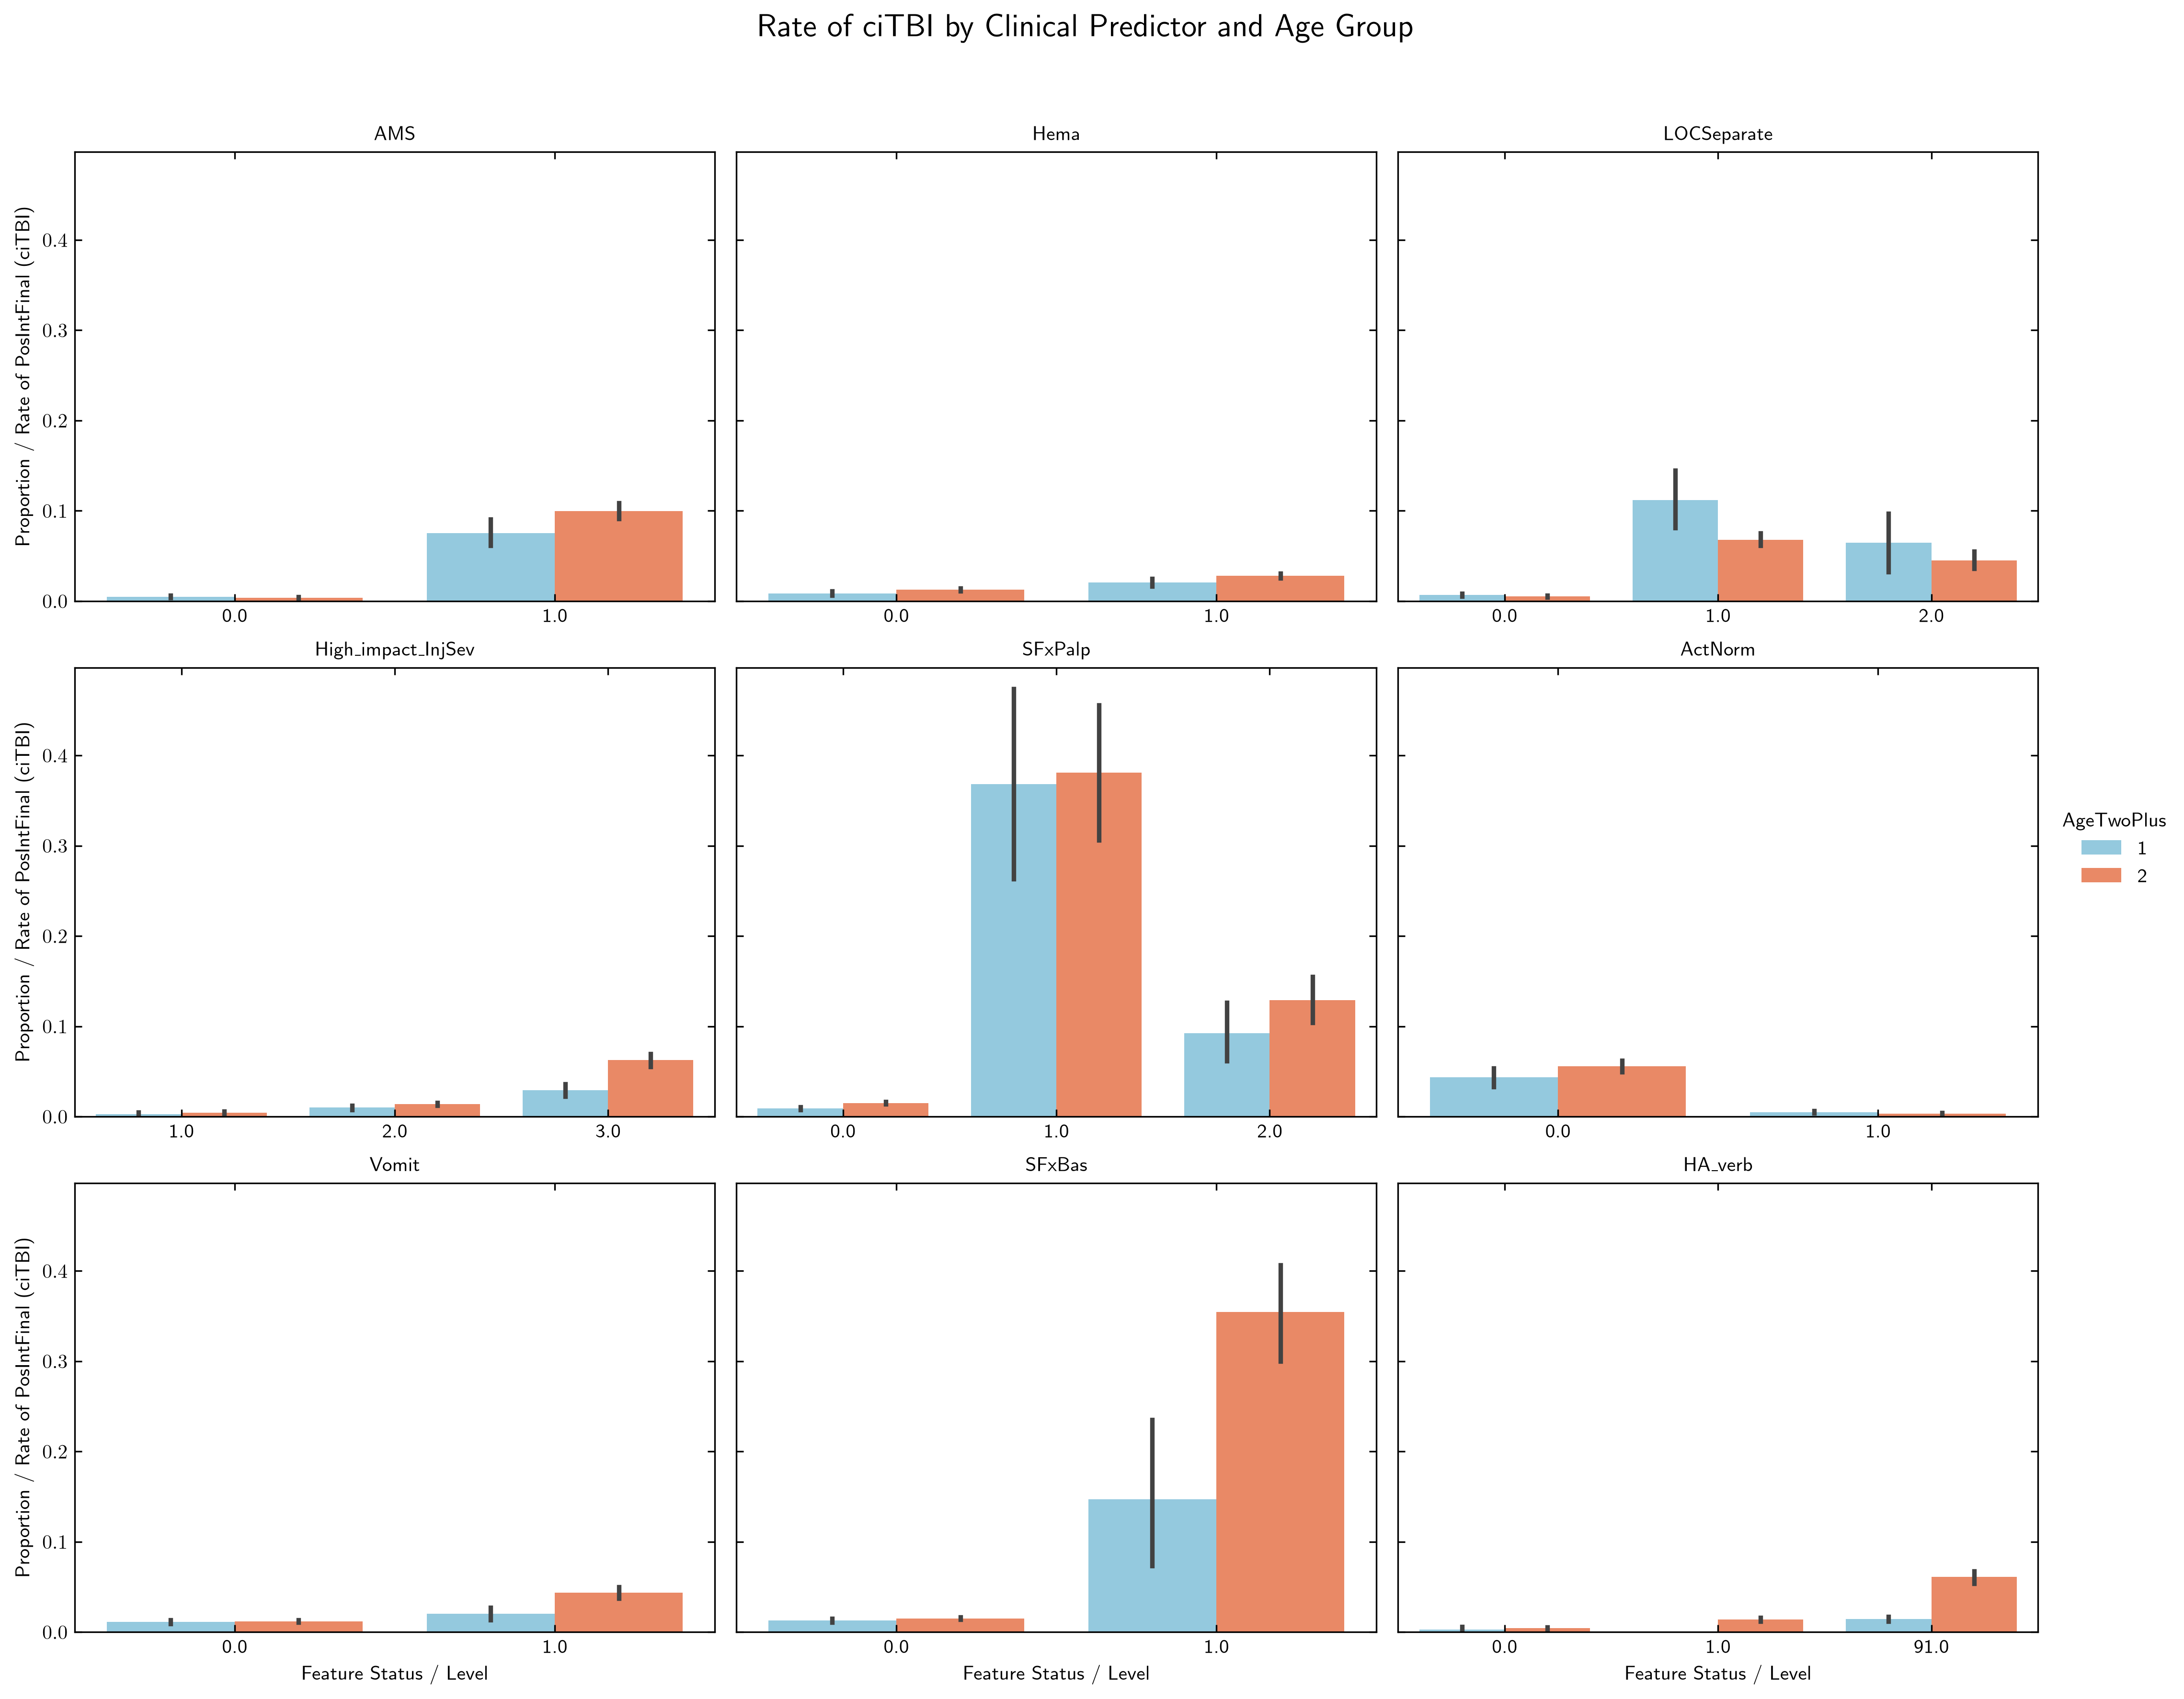
\includegraphics[width=\textwidth]{../figs/clinical_features_report.png}
\caption{Rate of ciTBI by Clinical Predictor and Age Group.}
\label{fig:clinical_features}
\end{figure}

\section{Findings}\label{findings}

When working with biological data, there are several complex relationships and interactions between variables that can be difficult to tease apart. In this section, I will present two interesting findings that were discovered during data exploration that are particularly relevant to the domain problem and establishing CDRs for pediatric head trauma. These findings are not necessarily novel, but are important to keep in mind later in the modeling stage.

\subsection{First finding}\label{first-finding}

When considering both age groups, one's first instinct might be to start by comparing the counts of ciTBI cases, as thus far the only distinction between CDRs were by age. However, we know it to be true that as children age, differences in the endocrine makeup between females and males become more pronounced, even prior to puberty, potentially creating misleading conclusions about the static ciTBI risk of being in a certain age group. Muenchhoff and Goulder [2] provide beautiful evidence of the biological basis for this phenomenon, driving home our understanding of the relationship between age and gender. This posed the question: as children age, do the rates of ciTBI differ between genders? To answer this question, both age groups were stratified by gender, providing evidence that there might be a distinct relationship between gender and risk for ciTBI in children at least 2 years old, results also seen in Sönnerqvist et al. [4].  It is worth noting that when considering children under the age of two, there is little to no difference between proportions of ciTBI rates between genders, but as children age, the difference, favoring males, become more pronounced. There are several explanations that one could attempt to give to explain this phenomenon, for example, someone could make the misguided claim that, traditionally, male children are more likely to engage in riskier, more dangerous behaviors than female children, but this is both only a speculative (not at all data driven, but bias driven) explanation and one that is quite sextist in nature. I make no such speculative claims about this relationship, as I am not an expert in pediatric endocrinology, still, this finding is important to consider when developing CDRs for pediatric head trauma.

\begin{figure}[h!]
\centering
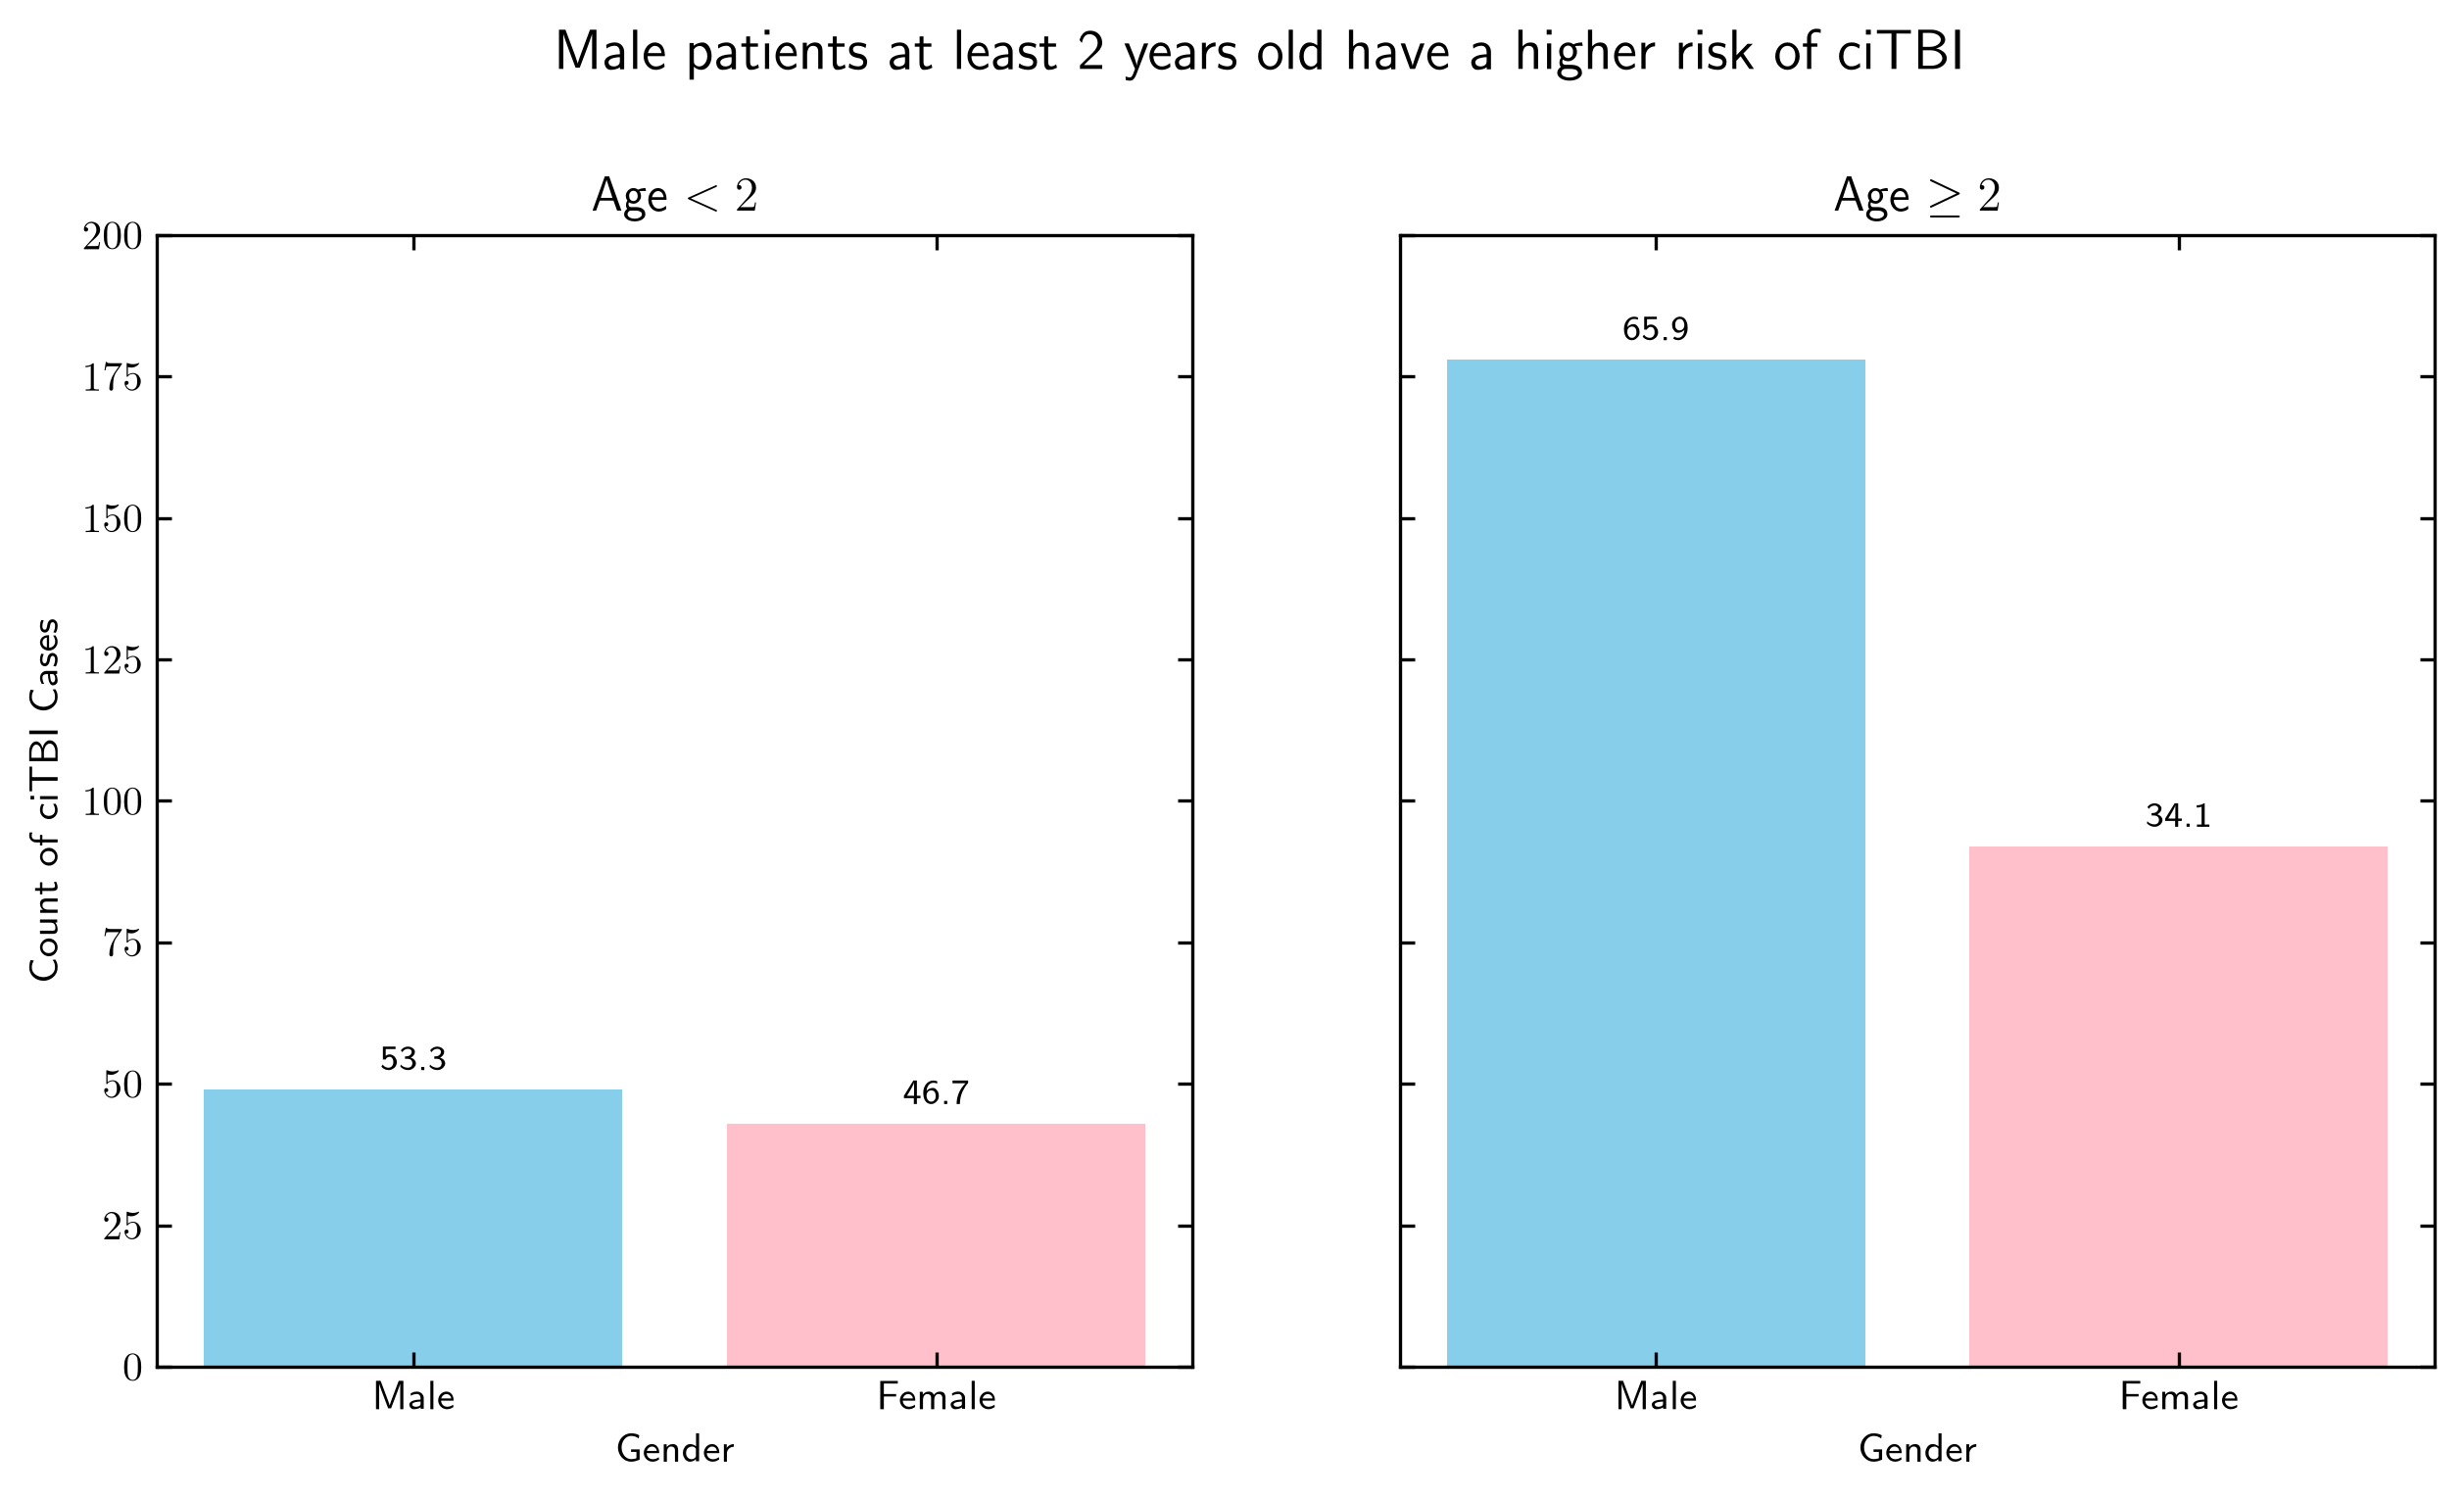
\includegraphics[width=0.95\textwidth]{../figs/finding_1.png}
\caption{Male patients at least 2 years old have a higher risk of ciTBI. (Right) The proportion of ciTBI cases for children under 2 years old stratified by gender. (Left) The proportion of ciTBI cases for children at least 2 years old stratified by gender.}
\label{fig:finding_1}
\end{figure}


\subsection{Second finding}\label{second-finding}

As noted in Ross et al. [3], there is evidence of racial disparities in the use of diagnostic imaging in the United States, prompting me to investigate this disparity in the PECARN data. It is of note that since this data is from specialized pediatric emergency departments, rather than general emergency departments, perhaps this disparity is not as pronounced, but it still worth investigating. 

\begin{figure}[h!]
\centering
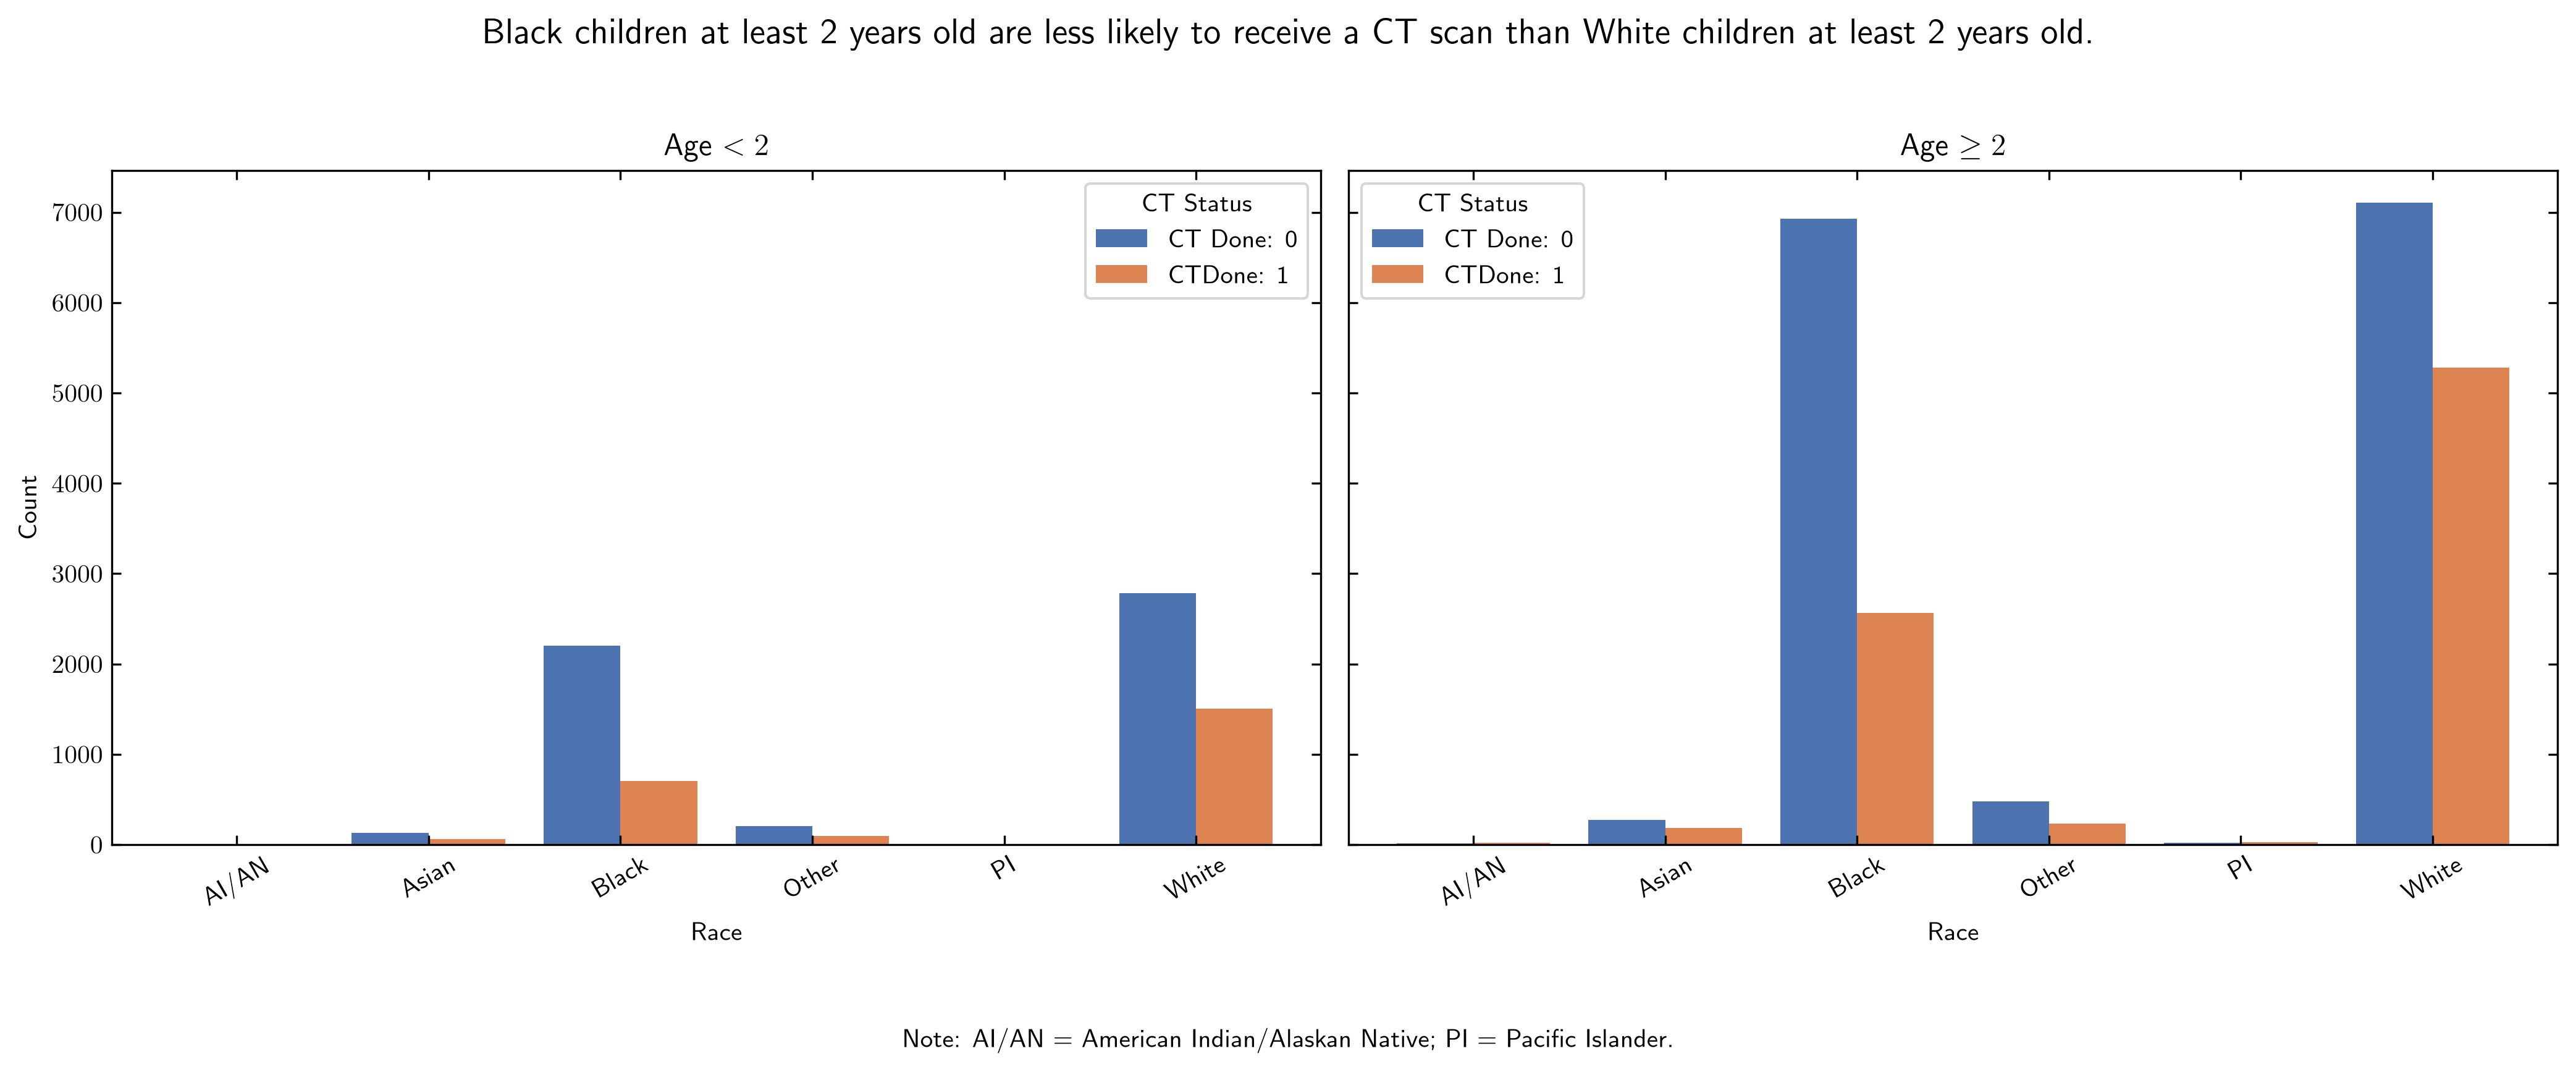
\includegraphics[width=0.95\textwidth]{../figs/finding_2.png}
\caption{Black children at least 2 years old are less likely to receive a CT scan than White children at least 2 years old. (Right) The proportion of \texttt{CTDone} for children under 2 years old stratified by gender. (Left) The proportion of \texttt{CTDone} for children at least 2 years old stratified by gender.}
\label{fig:finding_2}
\end{figure}

For both age groups, the proportion of Black children who received CT scans was lower than the proportion of White children who received CT scans, with the difference being much more pronounced in children at least two years old. Since the racial distributon of Black and White children is similar in both age groups, this suggests that the pronounced difference for children at least two years old is not simply due to a lack of Black children in one age group versus the other. Reasons for why this behavior might be observed are not clear, but it is worth noting that this finding is still apparent.

\subsection{Reality Check}\label{reality-check}

When considering the domain problem and how this data can answer our posed question, several assumptions must be made, and thus it is necessary to ground these assumptions in reality. For example, the assumption that this data is representative of the population of children who present to the emergency department with head trauma is one that we are trying to make, but in order to make such assumption, it is necessary to check that the data actually is representative of this population.

Several clinical variables recorded in this data, like \texttt{GCS}, are commonly recorded, of which we have extensive knowledge on, i.e. Glascow-Coma Scale scores range from 3 (severe) to 15 (mild). Thus, we can leverage this knowledge to check that the data variable \texttt{GCS} actually falls within this range. Recall that while this analysis was restricted to children with a GCS score of 14 or 15, patients with a smaller score were also eligble to participate, and thus data exists for such children. Upon looking at this rather trivial check, we see that it is in fact true that the range of \texttt{GCS} is what we expect, elimatining the possibility of severe data entry errors indicative of an unrepresentative data set.

It is also known that in determining loss of consciousness, there are three different categories a patient may fall into: no loss of consciousness, suspected loss of consciousness (presyncope), and confirmed loss of consciousness (syncope). One vital data cleaning step involved changing patients' \texttt{LOC} state from \texttt{Suspected} to \texttt{Yes} if they had a duration of loss of consciousness recorded. Consider the main difference between syncope and presyncope: syncope is a temporary loss of consciousness while presyncope is a state of lightheadedness, feeling faint, etc. If the patient, or someone attending the emergency department with the patient, has information regarding how long a certain event might have occurred, it is reasonable to assume that event occurred long enough/severe enough to make note of it, making their episode clinically meaningful in terms of determining ciTBI.

Recall, we separate our population into two subpopulations: under 2 and at least 2 years old. Simply due to the age of the patient, there are reasonable expectations of what the child's injury might have resulted from. For example, a child under 2 years old typically does not know how to ride a bike, and thus we would expected to see a very low proportion of such injuries, especially comparing with older children who are more likely to ride bikes. Table 5 summarizes the counts of injury type for both age categories. We see that this fact of nature is reflected in the data, also grounding this data in reality. The same logic applies to sports injuries --- children under 2 years old are not likely to be playing sports yet, especially publicly organized sports.

\begin{table}[htbp]
  \centering
  \begin{tabular}{l|c|c}
    \hline
    \textbf{Injury Mechanism} & \textbf{$<2$ years old} & \textbf{$\ge 2$ years old} \\
    \hline
    MVC & 197 & 2762 \\
    \hline
    Pedestrian & 41 & 991 \\
    \hline
    Bicycle Collision - Vehicle & \cellcolor{yellow!30}3 & 416 \\
    \hline
    Bicycle Collision - Other & \cellcolor{yellow!30}10 & 1299 \\
    \hline
    Other Crash & 37 & 628 \\
    \hline
    Fall - Standing & 768 & 2887 \\
    \hline
    Collision with Stationary Object & 472 & 1423 \\
    \hline
    Fall - Elevated & 4600 & 4630 \\
    \hline
    Fall - Stairs & 1186 & 1060 \\
    \hline
    Sports & \cellcolor{yellow!30}6 & 2228 \\
    \hline
    Assault & 55 & 2316 \\
    \hline
    Object - Accidental & 412& 2074 \\
    \hline
    Other & 602 & 2028 \\
    \hline
  \end{tabular}
  \caption{Injury Mechanism Data by Age Group}
  \label{tab:injury_mech}
\end{table}

\subsection{Stability Check}\label{stability-check}

As documented in the data cleaning section, there were several judgement calls made in terms of how to clean some of the variables: \texttt{LOC}, \texttt{AMS}, \texttt{InjurySev}. To compare the stability of the findings, I will compare one finding with its counterpart when the data is cleaned with the absence of such judgement calls. That is, when cleaning \texttt{AMS}, we cosider \texttt{GCS} as the sum of its components in the data and not simply \texttt{GCSTotal}, missing injury severity is not imputed for pedestrians, and \texttt{LOC} is not changed from \texttt{Suspected} to \texttt{Yes} if a duration of loss of consciousness is recorded.

\begin{figure}[h!]
\centering
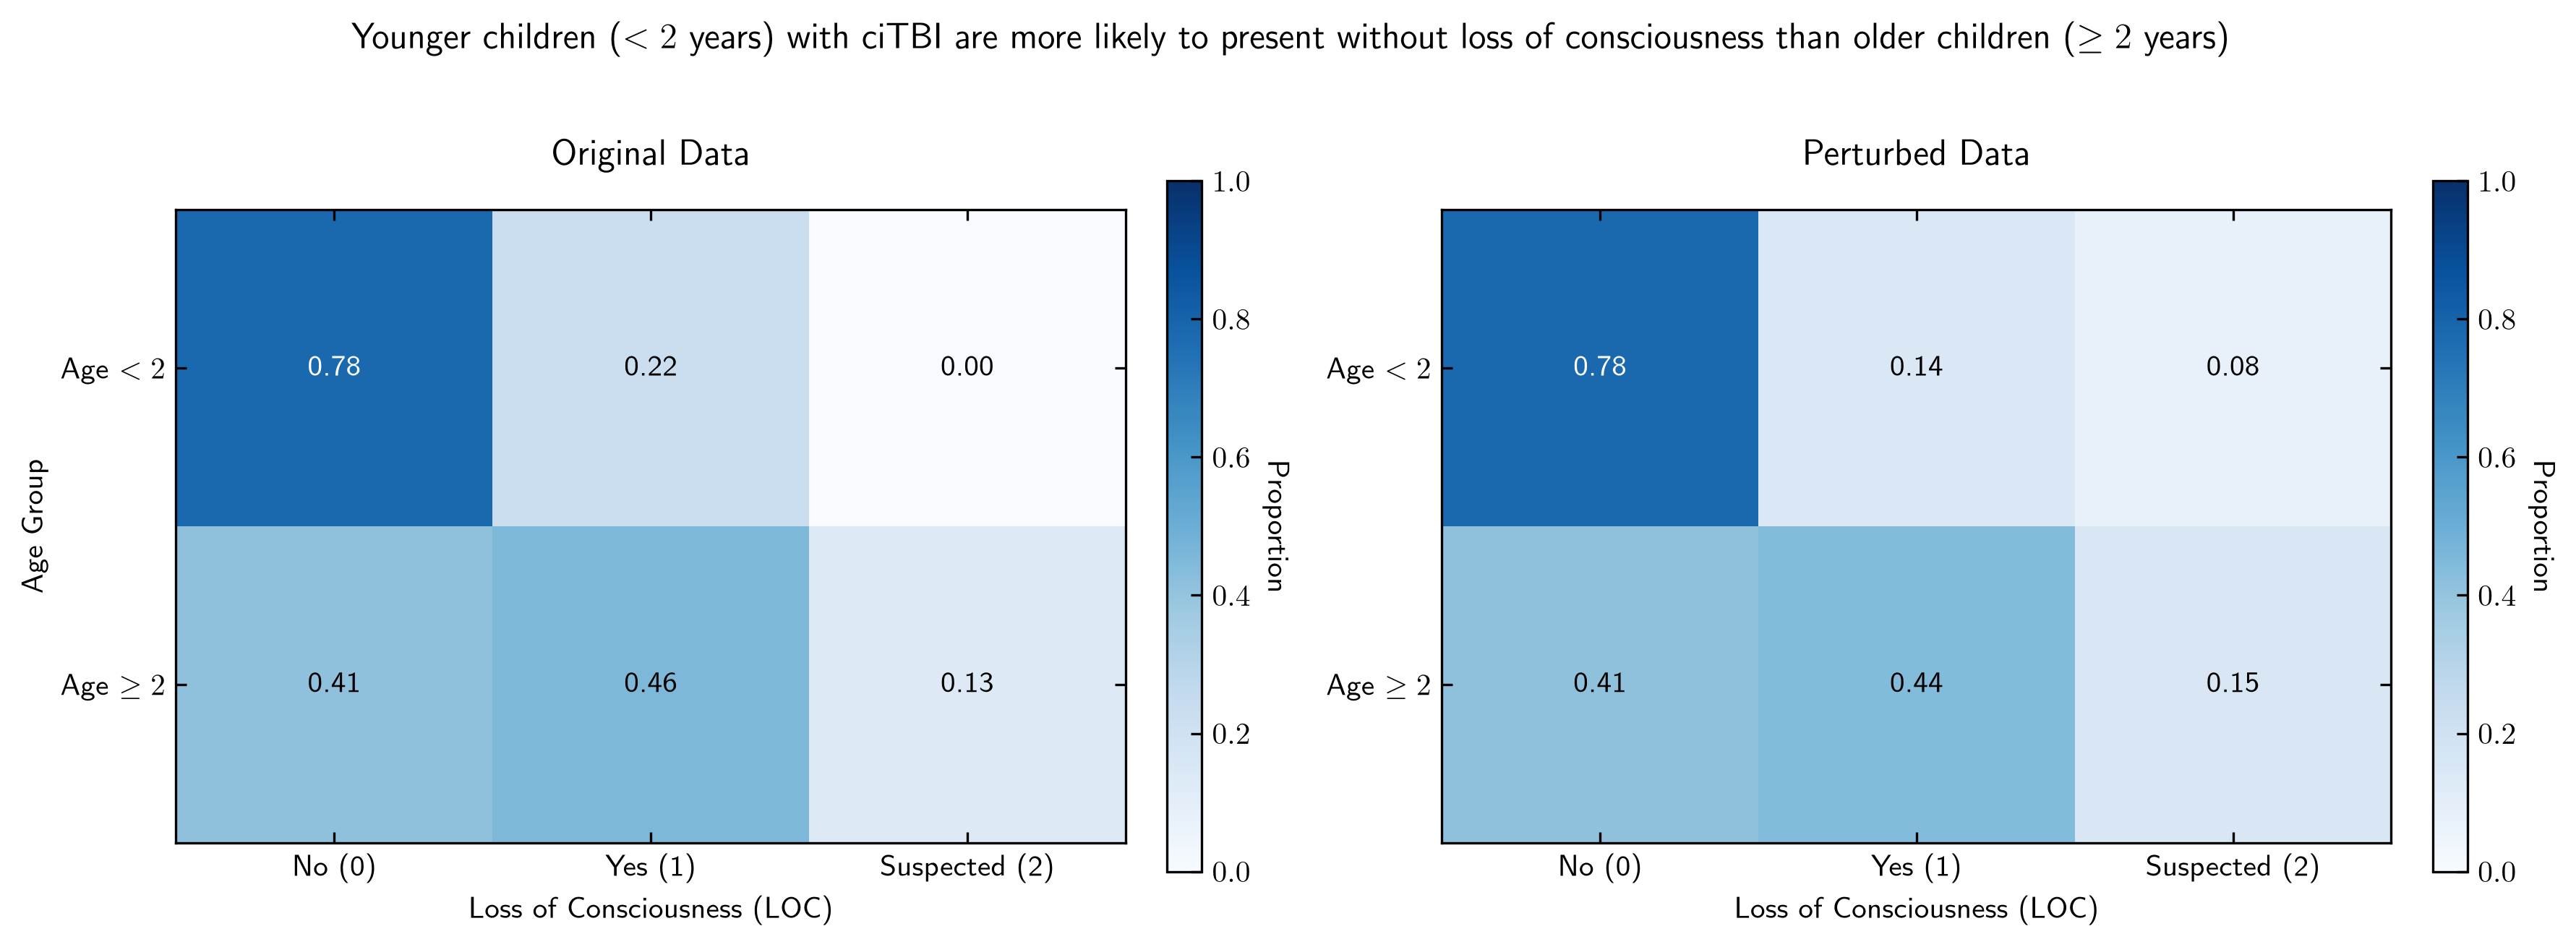
\includegraphics[width=0.95\textwidth]{../figs/findings_perturbed.png}
\caption{Younger children ($<2$ years old) with ciTBI are more likely present without loss of consciousness than older children ($\geq 2$ years old). (Right) Original data. (Left) Perturbed data.}
\label{fig:finding_2_perturbed}
\end{figure}

Several features were used in the orginal CDRs for both age groups, e.g., altered mental status, loss of consciousness, and high impact injury severity. Considering this shared ruled set, I began to ponder: do any of these features have a different relationship with ciTBI depending on the age group? As it turns out (see Figure 4), younger children ($<2$ years old) are more likely (higher proportion) to present to the emergency department without loss of consciousness than older children ($\geq 2$ years old). This suggests that the relationship of loss of consciousness with ciTBI is in fact different between the two age groups, and thus this observation should be kept in mind when developing CDRs for pediatric head trauma. Does this suggest that loss of consciousness is less important for older childen? Not necessarily! The data suggests that loss of consciousness is equally important in its own manner between the two age groups. Children under 2 years old who have loss of consciousness might have "stronger" evidence for ciTBI compared to children at least 2 years old, but evidence of loss of consciousness alone is a neurological concern that should not be ignored. The same relationship is observed under the perturbed data, suggesting that this finding is stable under data perturbation.


\section{Modeling}

For this report, as has been re-iterated throughout, the goal is to create Clincal Decision Rules (CRDs) for pediatric head trauma. We are attempting to make decisions on whether a patient should be given a CT scan based on the prediction of ciTBI, maximizing both sensitvity and negative prediction value (NPV). In fact, this report hopes to see if we can find simpler CDRs than established in Kuppermann et al. [1], while still maintaining high sensitivity and NPV. Specifically, we start with the same features identified in the orginal CDRs (all 9 features between both age groups, with the hopes of, again, showing both age groups have different rules) and gender, as pointed out in the findings section, gender might be an important feature to consider.

\subsection{Implementation}

The first consideration to be taken when choosing the models used in this report, I remind readers that missing values were not imputed, and kept as being clinically meaningful. That being said, models should be selected in such a manner that can handle missing values, and thus tree-based models are a natural choice. The two models used in this report are the Classification Tree Classifier and XGBoost Classifier. For both models, all hyperparameters were determined using 10-fold cross validaition on the training data, where the hyperparameters were selected by maximizing accuracy for the Classification Tree Classifier and the area under the receiver operating characteristic curve (AUC) for the XGBoost Classifier. Due to the imbalanced nature of the data (ciTBI is a rare event), the models were trained using a balanced class weight, which penalizes misclassifications of the minority class more heavily than misclassifications of the majority class. The models were evaluated using sensitivity and negative predictive value (NPV), as these metrics are most relevant to the domain problem of identifying children at very low risk of ciTBI.


\subsection{Stability}



\begin{table}[htbp]
\centering
\caption{Model Performance Metrics Across Original and Perturbed Datasets}
\label{tab:model_comparison}
\begin{tabular}{llcccc}
\toprule
\multirow{2}{*}{\textbf{Model}} & \multirow{2}{*}{\textbf{Subgroup}} & \multicolumn{2}{c}{\textbf{Original Data}} & \multicolumn{2}{c}{\textbf{Perturbed Data}} \\
\cmidrule(lr){3-4} \cmidrule(lr){5-6}
& & \textbf{Sensitivity} & \textbf{NPV} & \textbf{Sensitivity} & \textbf{NPV} \\
\midrule
\multirow{2}{*}{Decision Tree} 
  & Under 2 & 0.80952 & 0.99742 & 0.80952 & 0.99742 \\
  & Over 2  & 0.76923 & 0.99682 & 0.76923 & 0.99682 \\
\addlinespace
\multirow{2}{*}{XGBoost} 
  & Under 2 & 0.85714 & 0.99837 & 0.85714 & 0.99837 \\
  & Over 2  & 0.80000 & 0.99756 & 0.80000 & 0.99756 \\
\bottomrule
\end{tabular}
\end{table}

It is of note, running the models on the perturbed data picks the same predictors as the original data, and the performance metrics are identical. For features that were perturbed in the data cleaning process, as investigated in the exploration phase, these perturbations did not change the structure of the data and hence we are finding the same CDRs.

\subsection{Discussion}

One large advantage of using tree-based models is that they are extremely interpretable, and thus we can easily visualize the decision-making process of the model. Figure 5 shows the structure of the decision tree model for both age groups. The decision tree model for children under 2 years old has two splits: first, on altered mental status (\texttt{AMS}) and then on injury severity, while the decision tree model for children at least 2 years old has two different splits: first, on whether the child is acting normal and then on \texttt{AMS}. The XGBoost model is an ensemble of decision trees, and thus it is not as interpretable as a single decision tree, but we can still use feature importance to understand which features are most important in making predictions. In fact, for XGBoost, the most important features for both age groups are identical to those used in the decision tree model, suggesting that these features are indeed important for predicting ciTBI.

\begin{figure}[htbp]
\centering
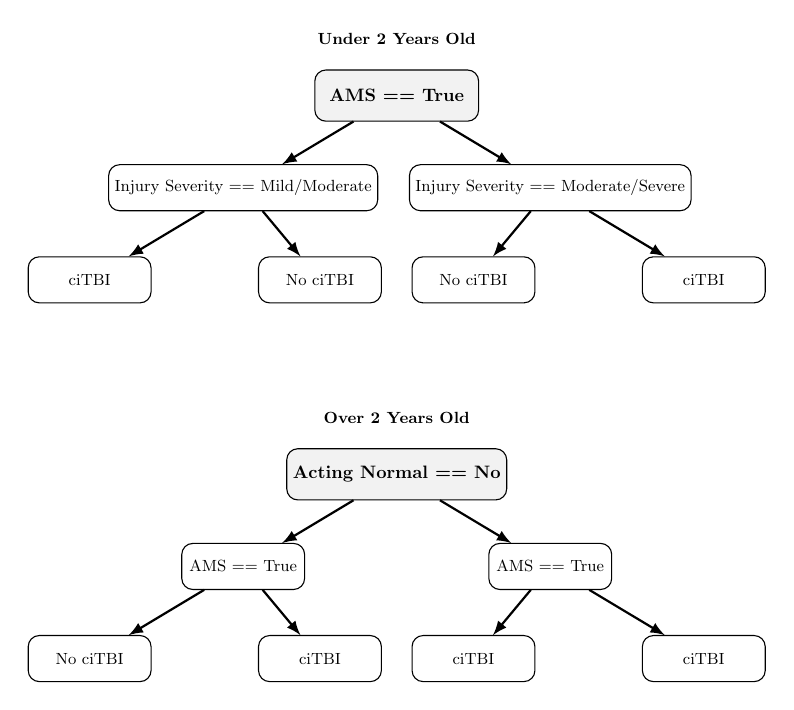
\begin{tikzpicture}[
    scale=0.65, transform shape,
    box/.style={draw, rectangle, rounded corners, minimum width=3.2cm, minimum height=1cm, align=center, fill=gray!10, font=\bfseries},
    subbox/.style={draw, rectangle, rounded corners, minimum width=2.4cm, minimum height=0.9cm, align=center, font=\small},
    line/.style={draw, -latex, thick}
]

    % Top: Decision Tree Model Structure -- under 2
    \node[align=center, font=\bfseries\small] at (0, 5.4) {Under 2 Years Old};
        
    \node[box] (dt_orig) at (0, 4.3) {AMS == True};
        
    \node[subbox] (dt_orig_u2) at (-3, 2.5) {Injury Severity == Mild/Moderate};
    \node[subbox] (dt_orig_o2) at (3, 2.5) {Injury Severity == Moderate/Severe};
        
    \node[subbox] (dt_orig_u3) at (-6, 0.7) {ciTBI};
    \node[subbox] (dt_orig_u4) at (-1.5, 0.7) {No ciTBI};
    \node[subbox] (dt_orig_o3) at (1.5, 0.7) {No ciTBI};
    \node[subbox] (dt_orig_o4) at (6, 0.7) {ciTBI};
        
    \draw[line] (dt_orig) -- (dt_orig_u2);
    \draw[line] (dt_orig) -- (dt_orig_o2);
    \draw[line] (dt_orig_u2) -- (dt_orig_u3);
    \draw[line] (dt_orig_u2) -- (dt_orig_u4);
    \draw[line] (dt_orig_o2) -- (dt_orig_o3);
    \draw[line] (dt_orig_o2) -- (dt_orig_o4);

    \node[align=center, font=\bfseries\small] at (0, -2.0) {Over 2 Years Old};
            
    \node[box] (dt_orig_b) at (0, -3.1) {Acting Normal == No};
            
    \node[subbox] (dt_orig_u2_b) at (-3, -4.9) {AMS == True};
    \node[subbox] (dt_orig_o2_b) at (3, -4.9) {AMS == True};
            
    \node[subbox] (dt_orig_u3_b) at (-6, -6.7) {No ciTBI};
    \node[subbox] (dt_orig_u4_b) at (-1.5, -6.7) {ciTBI};
    \node[subbox] (dt_orig_o3_b) at (1.5, -6.7) {ciTBI};
    \node[subbox] (dt_orig_o4_b) at (6, -6.7) {ciTBI};
            
    \draw[line] (dt_orig_b) -- (dt_orig_u2_b);
    \draw[line] (dt_orig_b) -- (dt_orig_o2_b);
    \draw[line] (dt_orig_u2_b) -- (dt_orig_u3_b);
    \draw[line] (dt_orig_u2_b) -- (dt_orig_u4_b);
    \draw[line] (dt_orig_o2_b) -- (dt_orig_o3_b);
    \draw[line] (dt_orig_o2_b) -- (dt_orig_o4_b);

\end{tikzpicture}
\caption{Decision Tree Model Structure for children in both age groups ($<2$ years and $\geq 2$ years).}
\label{fig:model_trees}
\end{figure}

As addressed in the stability check section, the models ran on both the original and perturbed data produced the same performance metrics, which is a good grounding to the stability of our model to small perturbations, but this doesn't address the question of whether or not either model performs better than the orginal CDRs. It is good to see that NPVs are relatively comparable between both the simpler and orginal CDRs. However, in clinical settings, rules like these should minimize missing patients who truly have ciTBI, thus it is not ethical to sacrifice sensitivity for simpler rules. That is, the recommendation is to continue using the original CDRs. That being said, the models used in this report are still useful for understanding some important relationships between features and ciTBI, and can be used to inform future CDRs.

\section{Conclusion}\label{conclusion}

The PECARN data set is very large, rich, and complex, providing a unique opportunity to explore the relationships between various clinical features and the risk of clinically important traumatic brain injury in children. The size of the data set allowed for a comprehensive analysis, but also presented challenges in terms of data cleaning and exploration. The extent of missingness in the data set posed a real challenge in terms of how to properly address it: just impute all missing values? Or, as I did, keeping the missing values as clinically meaningful? Although I am not a subject matter expert, the latter approach allowed for a more nuanced, data-driven understanding of the relationships between the features and the outcome.

Overall, the data set is rather representative of the population of children who present to the emergency department with head trauma, and thus the simpler rules identified in this report can be used in considering the importance of certain features in predicting ciTBI. The goal of the original study was to establish CT rules for pediatric patients so that radiation risk is reduced if unnecssary, which the paper does well to address. This report complements this work, but I find it important to note that the data set is specific to speciality pediatric hospitals, and thus the claim that CDRs will have a similar performance in general emergency departments is hard to make. Given information we have, this speculation is not unreasonable, but further work should be done to validate this hypothesis.

The lack of several necessary features in the data set, such as socioeconomic status, or even date of visit, makes it difficult to draw further claims about children in under-served areas as well as limits the ability to do appropriate data splitting for analysis. The modeling work done in this report does an excellent job at connecting the data-driven results to interpretabilty of the domain problem. While the simpler CDRs identified in this report are clincially meaningful and interpretable, I maintain that they should \textbf{not} replace the original CDRs established, as they sacrifice sensitivity for simplicity, which is not ethical in a clinical setting.

\section{Academic Honesty Statement}\label{academic-honesty-statement}

This statement is to affirm that the work presented in this report is original and my own. I assert that I have not received any unauthorize assistance in completing this work. All sources used to complete this report have been properly cited, both articles and individuals.

Academic honesty is  necessary and fundamental to the integrity of the academic community, as well as my own learning and development. Open science requires ownership of results and collaboration, ensuring reproduciblility and transparency. Acadmic integrity also covers plagarism. Plagarism is inherently against the views of good science, as 1$)$ it does not further any academic efforts and 2$)$ it violates trust that is necessary and curated within the academic and research communities.

\section{AI Disclosure}\label{ai-disclosure}

This statement discloses the use of artificial intelligence in the creation of this report:


This work utilized GitHub Copilot to assist with minor coding errors and typos. AI did not contribute to any of the analyses, interpretations, or generation of text used in this report. Google Gemini was used to convert tables to LaTeX format.

\section{Collaborators}\label{collaborators}

This work was completed in collaboration with the following students: Prithika Roy, Peter Zakariya, June Park, and Matt Eichner. The extent of the collabortion was solely discussion of the problem and the data. All code and analysis was completed independently.

\section{Bibliography}\label{bibliography}

 \begin{enumerate}[label={[\arabic*]}]
    \item Kuppermann, N., Holmes, J. F., Dayan, P. S., et al. (2009). Identification of children at very low risk of clinically-important brain injuries after head trauma: A prospective cohort study. The Lancet, 374(9696), 1160–1170. https://doi.org/10.1016/s0140-6736(09)61558-0.
    \item Muenchhoff, M., \& Goulder, P. J. R. (2014). Sex differences in pediatric infectious diseases. Nature Reviews Microbiology, 12(5), 338–350. https://doi.org/10.1038/nrmicro3235.
    \item Ross, A. B., Kalia, V., Chan, B. Y., \& Li, G. (2020). The influence of patient race on the use of diagnostic imaging in United States emergency departments: data from the National Hospital Ambulatory Medical Care survey. BMC Health Services Research, 20, Article 842. https://doi.org/10.1186/s12913-020-05698-1.
    \item Sönnerqvist, C., Brus, O., \& Olivecrona, M. (2020). Validation of the scandinavian guidelines for initial management of minor and moderate head trauma in children. European Journal of Trauma and Emergency Surgery, 47(4), 1163–1173. https://doi.org/10.1007/s00068-019-01288-x.
 \end{enumerate}

\end{document}
